\documentclass[a4paper, 10pt]{article}
\usepackage{../../CEDT-Homework-style}

\usepackage{amsmath}
\allowdisplaybreaks

\setlength{\headheight}{14.49998pt}

\begin{document}
\subject[2110203 - Computer Engineering Mathematics II]
\hwtitle{Signal 2}{}{Week 2}{6733172621 Patthadon Phengpinij}{ChatGPT (for\,\LaTeX\,styling and grammar checking)}


% ================================================================================ %
\section{Representing Signals}
% ================================================================================ %



% ================================================================================ %
%                                    Problem 01                                    %
% ================================================================================ %
\begin{problem}
Evaluate the convolution of the following signals
\end{problem}

% === Problem 1.1. === %
\begin{subproblems}[start=1]
    \item \( \textrm{rect} \paren{ \frac{t-a}{a} } * \delta (t-b) \)
\end{subproblems}

\begin{solution}
From the sifting property of the delta function, we have:
\[ f(t) * \delta(t - b) = f(t - b) \]

Applying this property to our problem, we get:
\[ \textrm{rect} \paren{ \frac{t - a}{a} } * \delta(t - b) = \textrm{rect} \paren{ \frac{(t - b) - a}{a} } = \textrm{rect} \paren{ \frac{t - (a + b)}{a} } \]

Thus, the result of the convolution is:
\[ \boxed{ \textrm{rect} \paren{ \frac{t - (a + b)}{a} } } \]

Using Python to verify this result, we can implement the convolution and plot the results.
The plot of the signal is shown below:
\begin{center}
    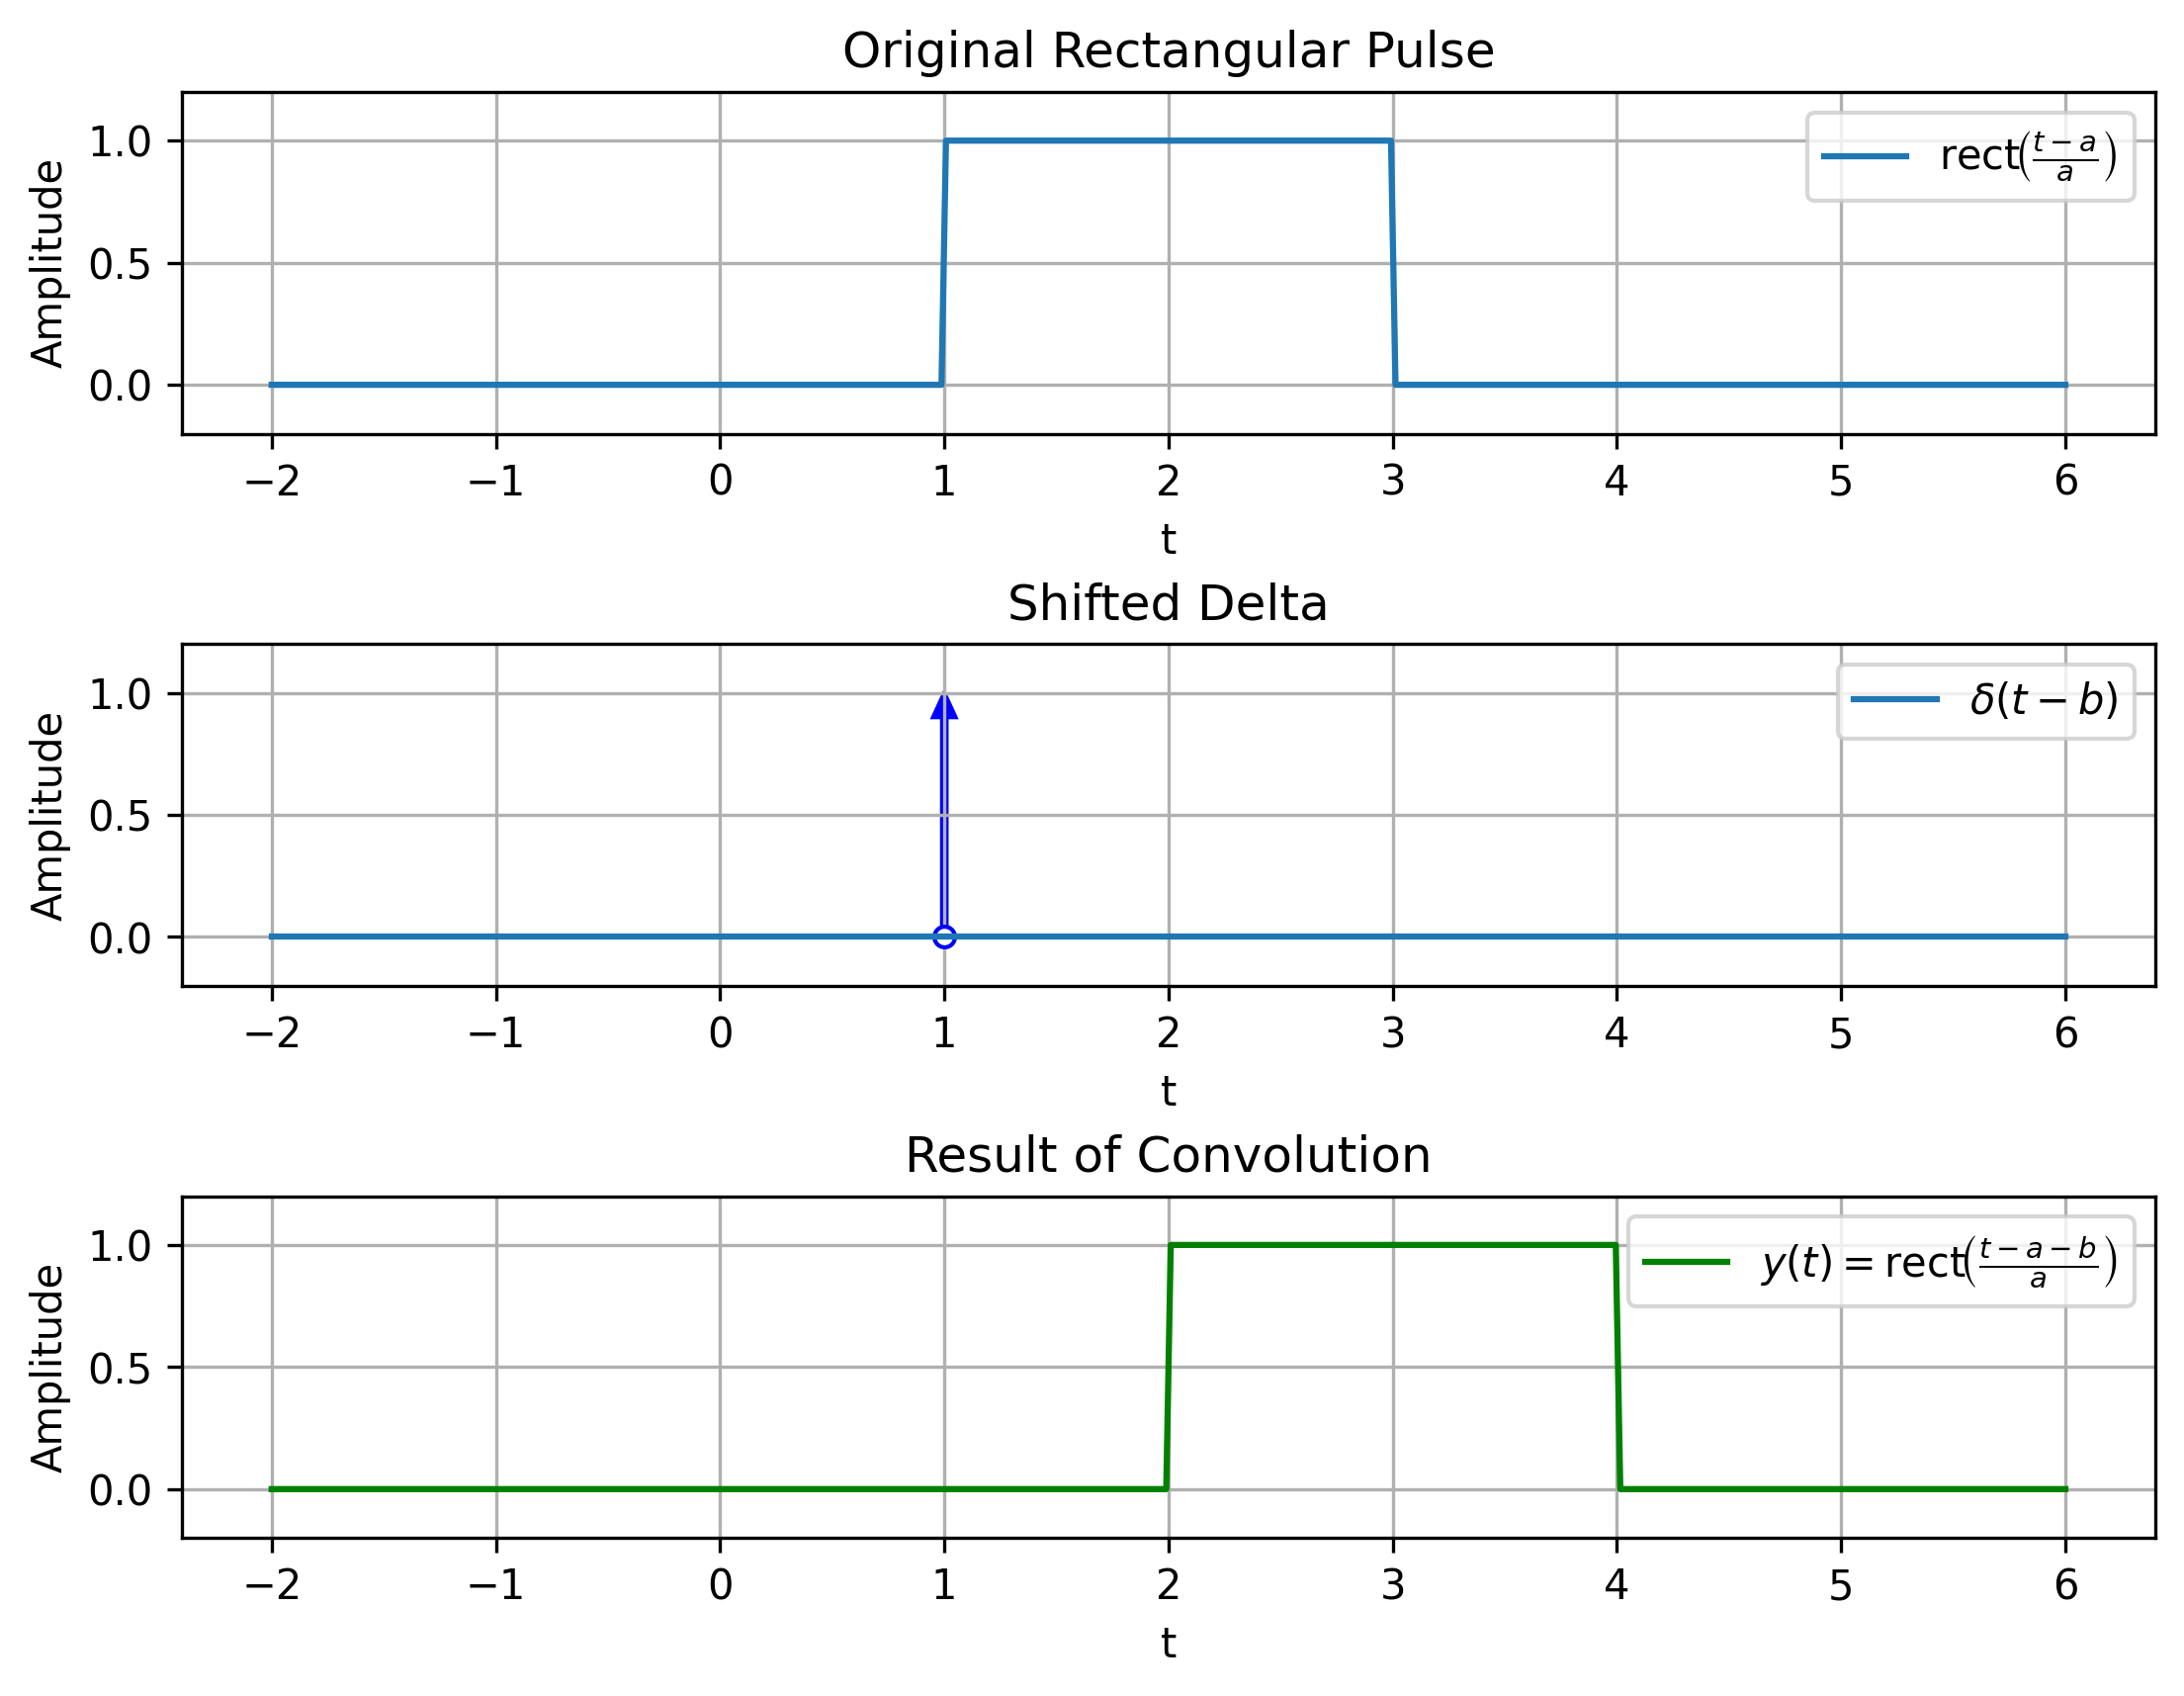
\includegraphics[width=0.8\textwidth]{images/problem_1_1.png}
\end{center}
\end{solution}
% ==================== %

\newpage

% === Problem 1.2. === %
\begin{subproblems}[resume]
    \item \( \textrm{rect} \paren{ \frac{t}{a} } * \textrm{rect} \paren{ \frac{t}{a} } \)
\end{subproblems}

\begin{solution}
To evaluate the convolution of two rectangular functions, we start with the definition of the rectangular function:
\[ \textrm{rect} \paren{ \frac{t}{a} } = \begin{cases} 1 & \text{if } |t| \leq \frac{a}{2} \\ 0 & \text{otherwise} \end{cases} \]

The convolution of two functions \( f(t) \) and \( g(t) \) is defined as:
\[ (f * g)(t) = \int_{-\infty}^{\infty} f(\tau) g(t - \tau) \, d\tau \]

Applying this to our rectangular functions, we have:
\[
\begin{aligned}
    ( \textrm{rect} \paren{ \frac{t}{a} } * \textrm{rect} \paren{ \frac{t}{a} } )(t) &= \int_{-\infty}^{\infty} \textrm{rect} \paren{ \frac{\tau}{a} } \textrm{rect} \paren{ \frac{t - \tau}{a} } \, d\tau \\
    &= \int_{-\frac{a}{2}}^{\frac{a}{2}} \textrm{rect} \paren{ \frac{t - \tau}{a} } \, d\tau \\
    &= \int_{\max(-\frac{a}{2}, t - \frac{a}{2})}^{\min(\frac{a}{2}, t + \frac{a}{2})} 1 \, d\tau \\
    ( \textrm{rect} \paren{ \frac{t}{a} } * \textrm{rect} \paren{ \frac{t}{a} } )(t) &= \min\left(\frac{a}{2}, t + \frac{a}{2}\right) - \max\left(-\frac{a}{2}, t - \frac{a}{2}\right)
\end{aligned}
\]

Evaluating the limits, we find that the result is a triangular function:
\[ \boxed{ \textrm{rect} \paren{ \frac{t}{a} } * \textrm{rect} \paren{ \frac{t}{a} } = \begin{cases} 
    0 & |t| > a \\
    t + a & -a \leq t < 0 \\
    a - t & 0 \leq t \leq a
\end{cases} } \]

Using Python to verify this result, we can implement the convolution and plot the results.
The plot of the signal is shown below:
\begin{center}
    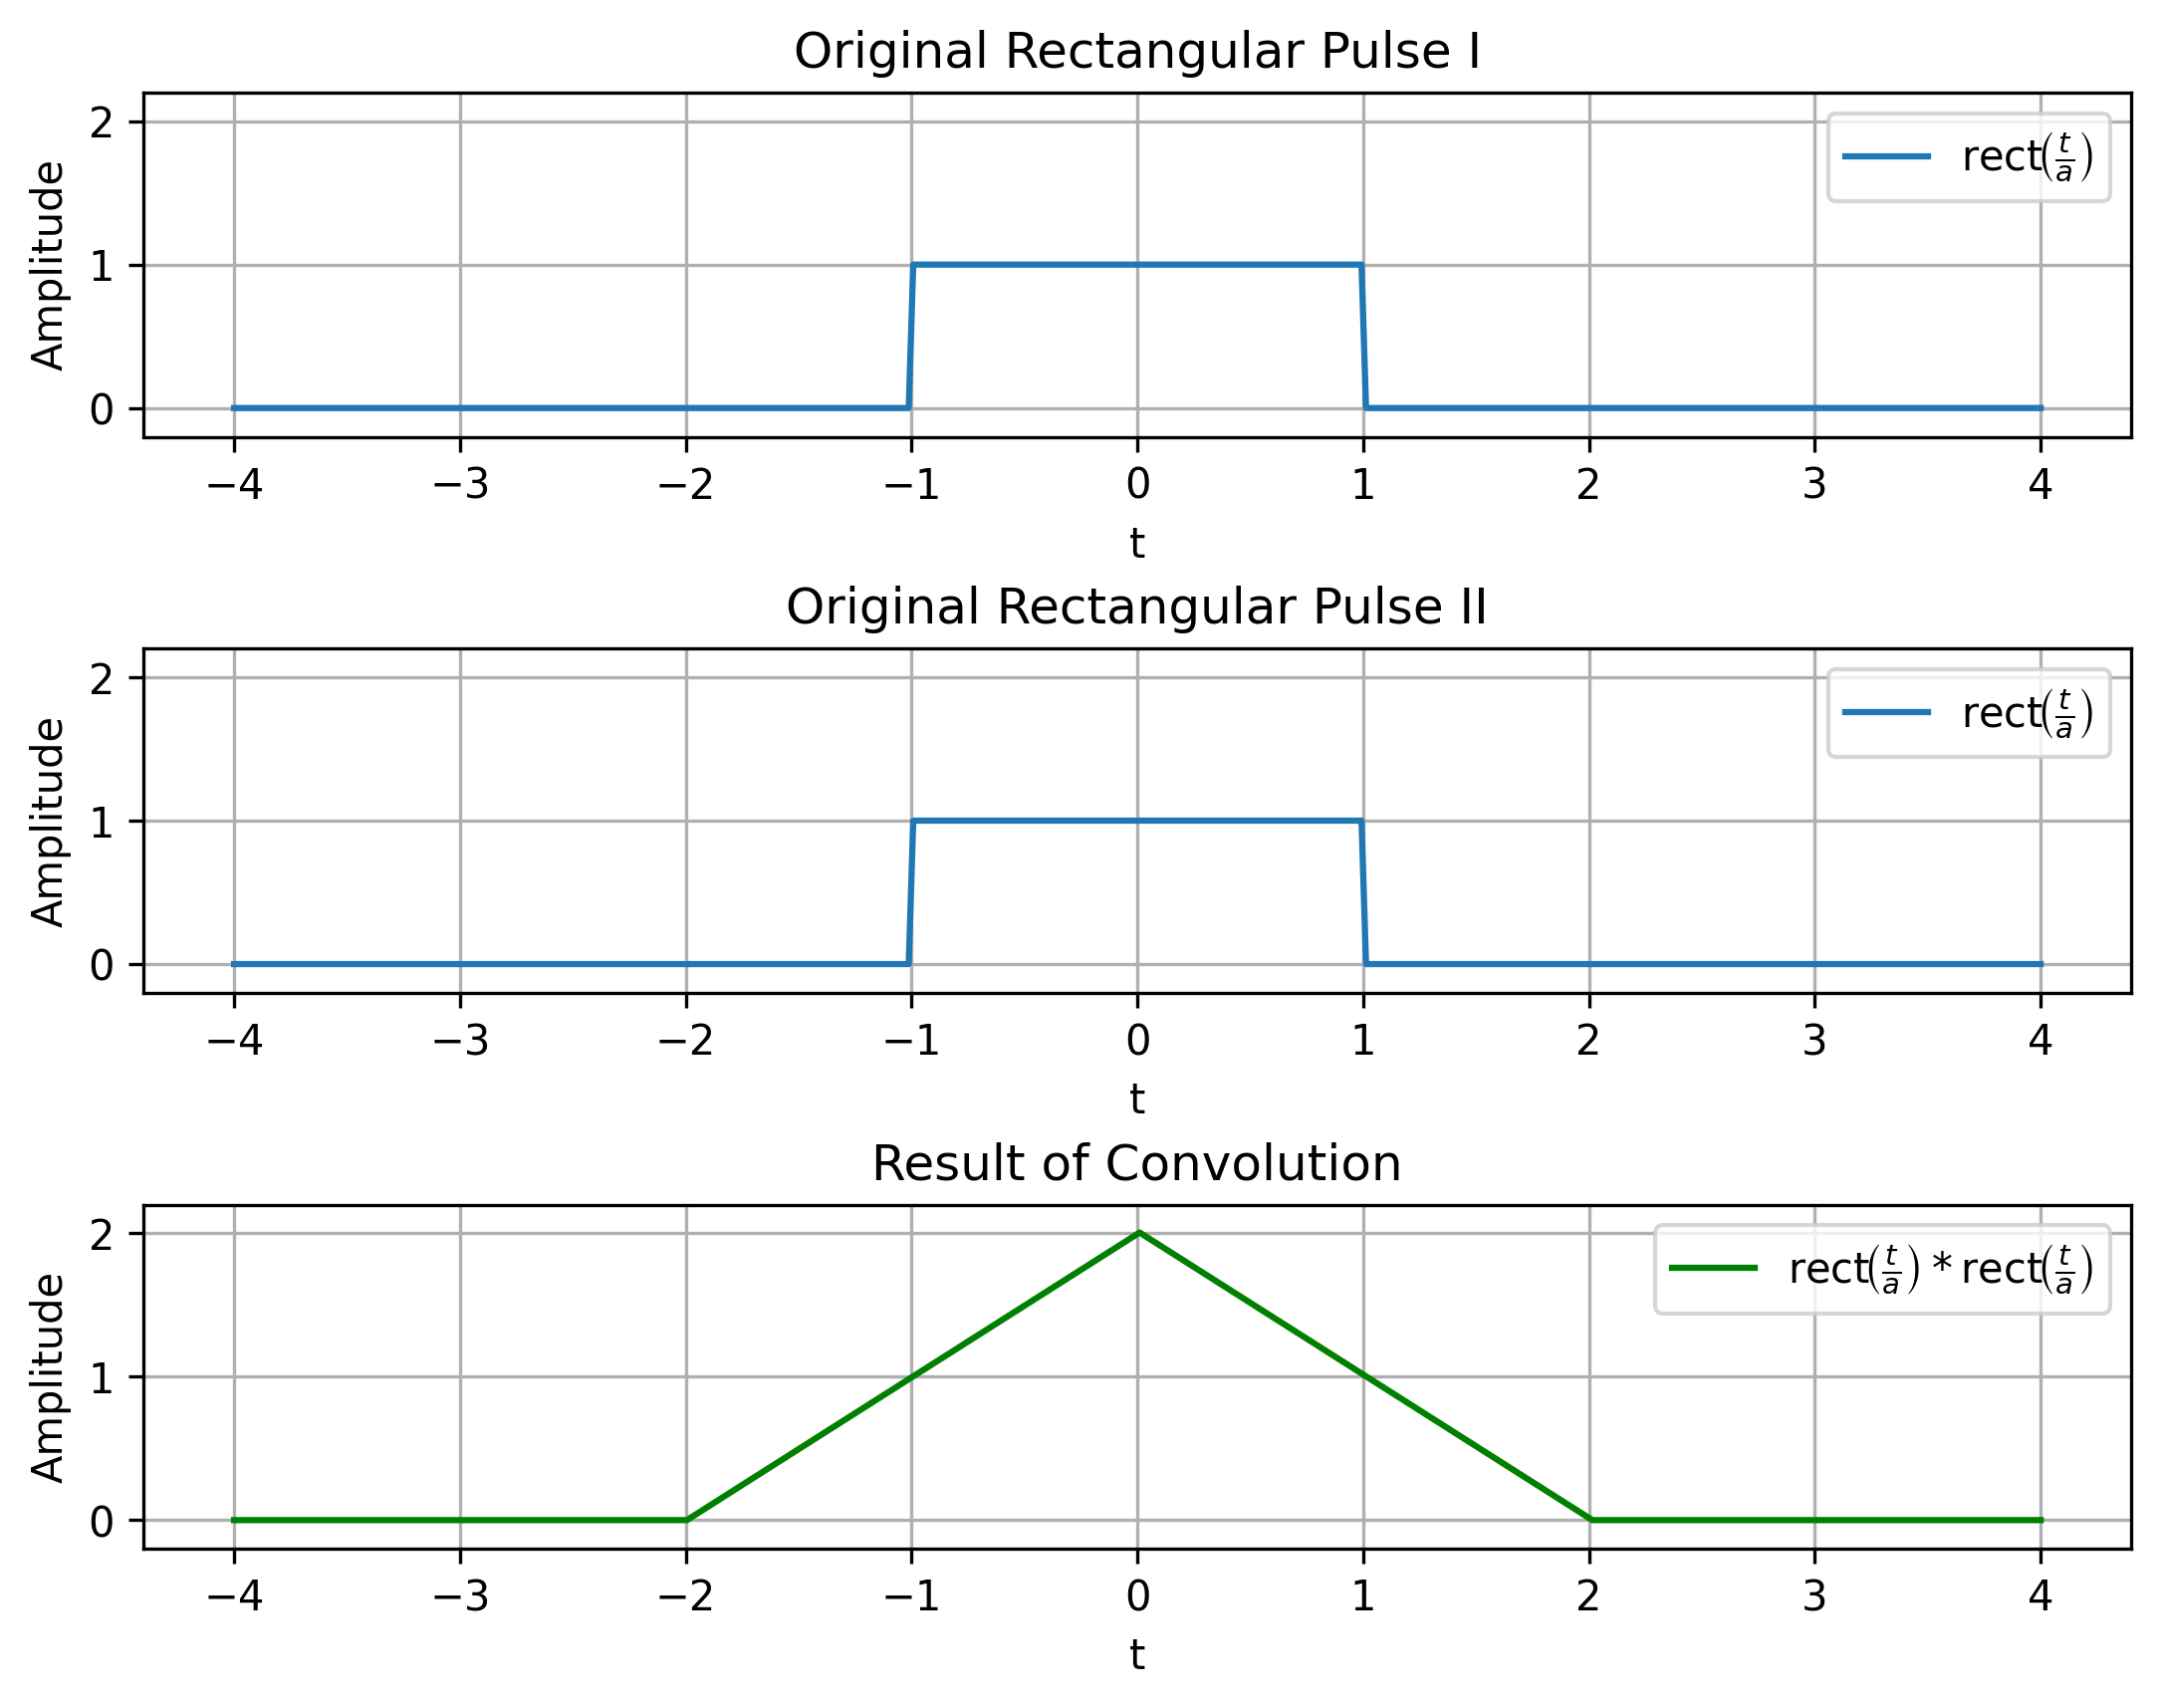
\includegraphics[width=0.8\textwidth]{images/problem_1_2.png}
\end{center}
\end{solution}
% ==================== %

\newpage

% === Problem 1.3. === %
\begin{subproblems}[resume]
    \item \( t[u(t)-u(t-1)]*u(t) \)
\end{subproblems}

\begin{solution}
First, we define the functions involved in the convolution:
\[ x(t) = t[u(t) - u(t-1)] = \begin{cases} 0 & t < 0 \\ t & 0 \leq t < 1 \\ 0 & t \geq 1 \end{cases} \]
\[ u(t) = \begin{cases} 0 & t < 0 \\ 1 & t \geq 0 \end{cases} \]

The convolution \( y(t) = x(t) * u(t) \) is given by:
\[ y(t) = \int_{-\infty}^{\infty} x(\tau) u(t - \tau) \, d\tau \]

Evaluating the convolution integral, we find:
\begin{align*}
    y(t) &= \int_{0}^{1} \tau \cdot u(t - \tau) \, d\tau \\
    y(t) &= \int_{0}^{\min(t, 1)} \tau \, d\tau
\end{align*}

Thus,
\[ \boxed{
y(t) = \begin{cases} 
    0 & t < 0 \\
    \frac{t^2}{2} & 0 \leq t < 1 \\
    \frac{1}{2} & t \geq 1
\end{cases}
} \]

Using Python to verify this result, we can implement the convolution and plot the results.
The plot of the signal is shown below:
\begin{center}
    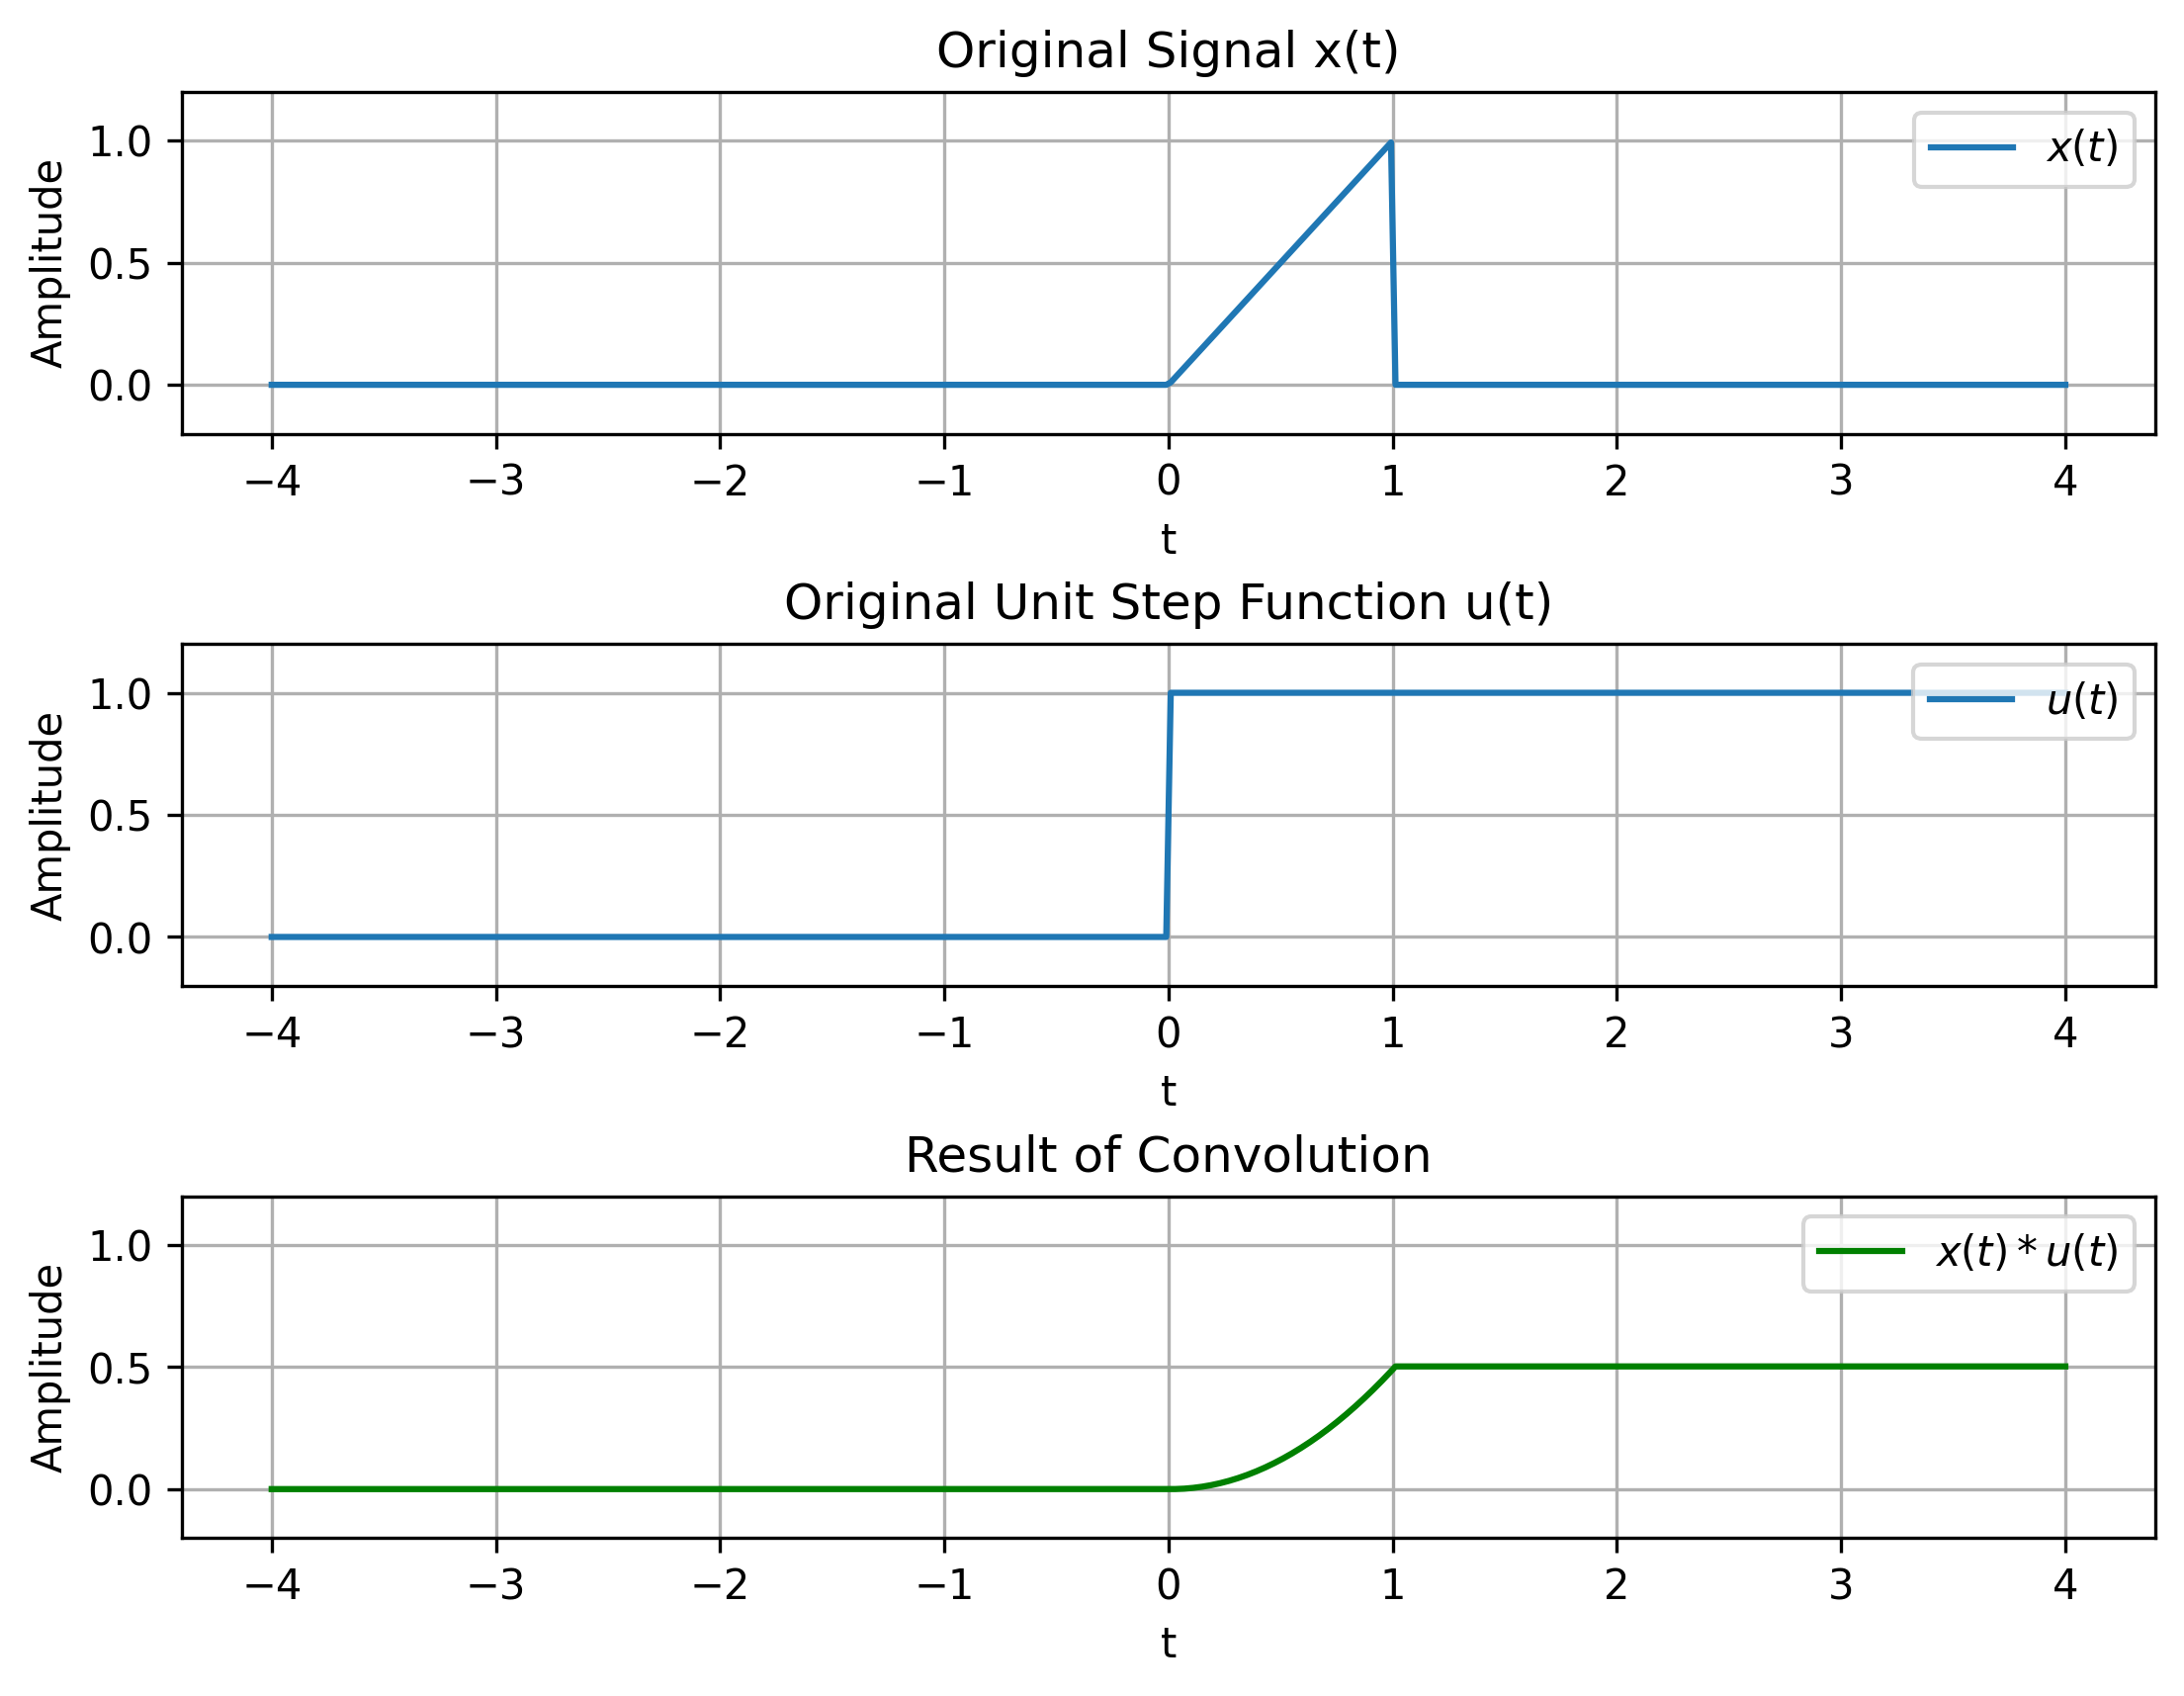
\includegraphics[width=0.8\textwidth]{images/problem_1_3.png}
\end{center}
\end{solution}
% ==================== %
% ================================================================================ %


\end{document}